\section{Benchmarking  for automated tuning and regression testing}\label{sec:bench}
%
Benchmarking was introduced in \linbox for several reasons. First, It 
gives the user a convenient way to produce quality graphs without 
of a graphing library like \gnuplot
\footnote{\url{http://www.gnuplot.info/}}
%
and provides the \linbox website with automatically updated tables and graphs.
Second, it can be used for regression testing.  Finally, it will be used for
selecting default methods and setting thresholds in installation time autotuning. % A lot of libraries do some automatic tuning
%at installation (\textsf{fftw}, \textsf{ATLAS}, \textsf{NTL},\ldots).
%
\par
%
% What do we do differently ? Selection between "larger" algorithms, takes more time.
% Interpolation.
% XXX BTL\footnote{\url{http://projects.opencascade.org/btl/}}/eigen
%
%
\subsection{Performance evaluation and Automated regression testing}
%
Our plotting mechanism is based on two structures: {\tt PlotStyle} and {\tt
PlotData}. The  {\tt PlotGraph} structure uses the style and data to manage the
output.  We allow plotting in standard image formats, html and \LaTeX tables,
but also in raw csv or xml for file exchange, data comparisons and
extrapolation. This mechanism can also automatically update \linbox feature
matrix that describes how our solutions behave on the fields we support. (vague)
% \danger dave benchmark formats discussion ?
%
\par
%
% \begin{figure}[htbp]
	\centering
	\small
	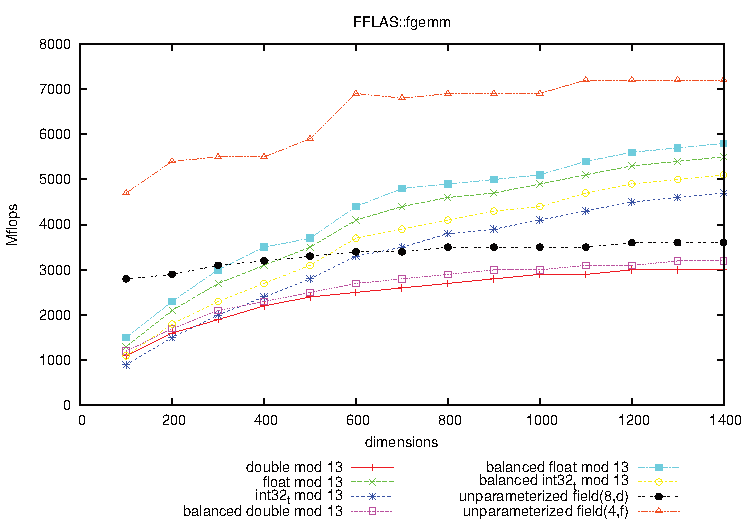
\includegraphics[scale=0.6]{Boyer_Brice/fgemm_square_13_ok}
	\caption{Example of \texttt{benchmark}: \texttt{fgemm}.\label{fig:bench}}
\end{figure}


%
% XXX Time spent on each data is limited (will not start execution if fit
% (linear least squares) forecasts 'too long'.\\
%
% XXX Adapts to the environment.
%
Saving graphs in raw format can enable automatic regression testing on the
buildbots that already checked our code. For some specifically determined matrices (of
various shapes and sizes and over several fields), we can accumulate the timings
for key solutions such as ({\tt rank}, {\tt det}, {\tt mul},\ldots) over time.
At each new release, when the documentation is updated, we can check any
regression on these base cases and automatically update the regression plots.
% \danger We need to implement this framework (not difficult; anybody?).
%JGD: we already have the buildbot, lets focus on this right now
%
\subsection{Automated tuning and method selection}
%
Some of the code in \linbox is already automatically tuned (such as thresholds
in \fgemm), but we improve on it. 
%It is well known that CPU throttling while

%building ATLAS causes bad optimizations; the \fflasffpack library could also

%suffer from not very reliable threshold detection (up to $50\%$ relative

%difference for some thresholds between runs). 
Instead of searching for a
threshold using fast dichotomous techniques, for instance, we propose to
interpolate curves and find the intersection. Using least squares fitting, we
may even tolerate outliers (but this is time consuming).
%JGD: there is already optimizer/winograd.C etc.
%
\par
%
Automatically tuning a library is not only about thresholds, it may 
also involve method/algorithm selection. Our strategy is the following: a given
algorithm is tuned for each {\tt Helper} (method) it has.  Then the solution
(that uses these algorithms) is tuned for selecting the best methods.  At each
stage, defaults are given, but can be overridden by the optimizer. The areas
where a method is better are extrapolated from the benchmark curves.
